\documentclass{beamer}

\usepackage{listings}
\usepackage{color}
\usepackage{inconsolata}
\usepackage{tikz}
\usepackage{hyperref}

%OL%\newcommand{\titleimage}{KeYBeamer2}
%OL%\usetheme{kit}
\beamertemplatenavigationsymbolsempty

\definecolor{mygreen}{rgb}{0,0.6,0}
\definecolor{mygray}{rgb}{0.5,0.5,0.5}
\definecolor{mymauve}{rgb}{0.58,0,0.82}


\newcommand{\KeY}{Ke\kern-.1em Y}
\newcommand{\kit}[1]{\textcolor{kit-green100}{#1}}
\newcommand{\kitblue}[1]{\textcolor{kit-blue100}{#1}}


\lstset{ 
  backgroundcolor=\color{white},   % choose the background color; you must add \usepackage{color} or \usepackage{xcolor}; should come as last argument
  basicstyle=\tiny\ttfamily,               % the size of the fonts that are used for the code
  breakatwhitespace=false,         % sets if automatic breaks should only happen at whitespace
  breaklines=true,                 % sets automatic line breaking
  captionpos=b,                    % sets the caption-position to bottom
  commentstyle=\color{mygreen},    % comment style
  deletekeywords={...},            % if you want to delete keywords from the given language
  escapeinside={\%*}{*)},          % if you want to add LaTeX within your code
  extendedchars=true,              % lets you use non-ASCII characters; for 8-bits encodings only, does not work with UTF-8
  %firstnumber=1000,                % start line enumeration with line 1000
  frame=single,	                   % adds a frame around the code
  keepspaces=true,                 % keeps spaces in text, useful for keeping indentation of code (possibly needs columns=flexible)
  keywordstyle=\color{blue},       % keyword style
  language=Java,                 % the language of the code
  alsoletter={\\},
  morekeywords={*,invariant,\\forall,requires,ensures,normal_behaviour,ghost,\\old,\\result,assignable},            % if you want to add more keywords to the set
  %numbers=left,                    % where to put the line-numbers; possible values are (none, left, right)
  numbersep=5pt,                   % how far the line-numbers are from the code
  %numberstyle=\tiny\color{mygray}, % the style that is used for the line-numbers
  rulecolor=\color{black},         % if not set, the frame-color may be changed on line-breaks within not-black text (e.g. comments (green here))
  %showspaces=false,                % show spaces everywhere adding particular underscores; it overrides 'showstringspaces'
  %showstringspaces=false,          % underline spaces within strings only
  %showtabs=false,                  % show tabs within strings adding particular underscores
  %stepnumber=2,                    % the step between two line-numbers. If it's 1, each line will be numbered
  %stringstyle=\color{mymauve},     % string literal style
  %tabsize=2,	                   % sets default tabsize to 2 spaces
  %title=\lstname                   % show the filename of files included with \lstinputlisting; also try caption instead of title
  deletecomment={[l]//},%
  deletecomment={[s]{/*}{*/}},%
}


\title{The \KeY-verified Verified Keyserver}

\date{27 April 2020}
\author[de Gouw, Ulbrich, Weigl]%
  {Stijn de Gouw (Open University, NL),
   Mattias Ulbrich, Alexander Weigl}

\institute{Institute of Theoretical Informatics}

\begin{document}

%OL%\selectlanguage{english}

\begin{frame}
\titlepage
\end{frame}

\begin{frame}{Our program verifier \KeY}
  \vspace{-1.5cm}
  \begin{center}
    \begin{tikzpicture}
      \node at (0,0) { 
\includegraphics[height=8cm]{key} };
      \node at (-2.5,2.5) {\large Deductive verification};
      \node[text width=3cm] at (-4.5,.5) {\large Java Modeling\\Language (JML)};
      \node[text width=3cm] at (4,-1.5) {\large Modular\\Reasoning};
      \node at (-3.5,-1.5) {\large Mostly automatic};
      \node at (2,2.5) {\large 100\% Java Card};
      \node at (-2,-2.5) {\large User Interaction Concepts};
      %\node at (2,-3) {\large Secure Information Flow};
      \node at (0,-4) {\footnotesize collaboration with
        TU Darmstadt and Chalmers University, Gothenburg};
    \end{tikzpicture}
  \end{center}\vspace{-1ex}
\end{frame}

\begin{frame}
  \frametitle{Modelling HAGRID in \KeY}

  We present two formalisations of the HAGRID framework as spec'ed and
  verif'ed Java implementations:
  \pause
  
  \begin{block}{The \textbf{array} model}
%  \footnotesize
    \begin{itemize}
    \item uses arrays to implement database and open requests
    \item specification on these arrays
    \item 70 loc, 90 los, 10 POs, \textbf{fully automatic}
    \end{itemize}
  \end{block}

  \only<1-2>{\it\footnotesize loc/los = lines of code/spec, POs = \# of
    proof obligations}
    
  
  \pause
  \begin{exampleblock}{The \textbf{map} model}
%  \footnotesize
  \begin{itemize}
    \item uses map data structures to implement db and open requests
    \item specification on ADT maps
    \item ``object singularities''
    \item 146 loc, 262 los, 40 POs, \textbf{89 interactions}
    \end{itemize}
  \end{exampleblock}
  % \tikz[overlay, text width=10cm] \node at (11.7,2) {\it\footnotesize loc/los = lines of code/spec\\POs = \# of proof obligations};
  
\end{frame}

\section{The array model: The class }
\begin{frame}
    \frametitle{The array model}
    \begin{columns}
    \begin{column}{.4\textwidth}
        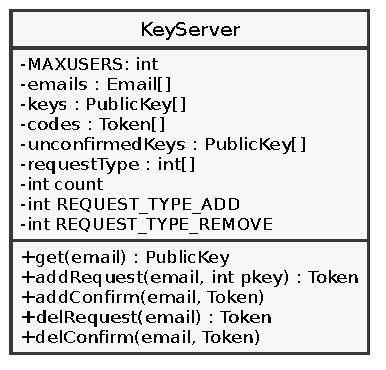
\includegraphics[width=\textwidth]{simplified_uml.pdf}
    \end{column}
    \begin{column}{.6\textwidth}
        \begin{itemize}
            \item Backend of Hagrid
            \begin{itemize}
                \item retrieving of public keys
                \item verified adding of entries
                \item verified deletion of entries
            \end{itemize}
            \item Simplifications
            \begin{itemize}
                \item All data types are (array of) \texttt{int}'s.
                \item Maps are represented by a key/value array.
            \end{itemize}
            \item \href{https://github.com/KeYProject/verifythis-ltc-2020/blob/master/simplified/Keyserver.java}%
                        {simplified/Keyserver.java}
        \end{itemize}
    \end{column}
    \end{columns}
\end{frame}

\begin{frame}[fragile]
    \frametitle{The array model: Invariants}
    
  \begin{block}{\small ruling out aliasing}
    \begin{lstlisting}
invariant emails != keys && emails != codes && emails != unconfirmedKeys;
invariant emails != requestType;
invariant keys != codes && keys != unconfirmedKeys;
invariant keys != requestType;
invariant codes != unconfirmedKeys && codes != requestType;
invariant unconfirmedKeys != requestType;\end{lstlisting}
  \end{block}
  \vspace{-1em}
  \begin{block}{\small All arrays are non-null and have the same length (the # users)}
\begin{lstlisting}
invariant emails != null && keys != null && codes != null;
invariant unconfirmedKeys != null && requestType != null;
invariant emails.length == MAXUSERS && keys.length == MAXUSERS;
invariant codes.length == MAXUSERS && unconfirmedKeys.length == MAXUSERS;
invariant requestType.length == MAXUSERS;\end{lstlisting}
  \end{block}
  \vspace{-1em}
  \begin{block}{\small number of users is bounded}
\begin{lstlisting}
invariant 0 <= count && count <= MAXUSERS;\end{lstlisting}
  \end{block}
  \vspace{-1em}
\begin{block}{\small emails are unique}
\begin{lstlisting}  
invariant (\forall int i,j ; 
                0 <= i && i < j && j < count; 
                    emails[i] != emails[j]);\end{lstlisting}
  \end{block}
\end{frame}

\begin{frame}[fragile]
    \frametitle{The array model: a method contract}
    \begin{block}{Informal Contract: \texttt{add(Email, PublicKey)}}
      Stores request to add the given key for the specified user. The key still
      needs to be confirmed with \texttt{#addConfirm(Email, Token)}. Does nothing if
      the specified user does not exist.
     
    \begin{itemize}
    \item \texttt{id} the email of the user
     \item \texttt{pkey}  -- public key to added after confirmation
     \item \textbf{returns} the array index where the key will be stored
    \end{itemize}
     
    \end{block}
    
    \begin{lstlisting}
    public int addRequest(int id, int pkey) {
        int pos = posOfId(id);  // find the entry in the current
        if(pos < 0) { pos = count++; } // not found, use an empty entry
        emails[pos] = id;
        codes[pos] = random(); 
        unconfirmedKeys[pos] = pkey;
        requestType[pos] = REQUESTTYPE_ADD;
        return pos;
    }
    \end{lstlisting}
\end{frame}

\begin{frame}[fragile]
    \frametitle{The array model: \texttt{addConfirm}}
\begin{lstlisting}
public normal_behaviour
requires count < MAXUSERS;      // internal capacity limit not reached
ensures 0 <= \result;           
ensures count == \old(count) && \result < count
     ||  count == \old(count) + 1 && \result == count - 1;
ensures emails[\result] == id && unconfirmedKeys[\result] == pkey && codes[\result]>0;
ensures requestType[\result] == REQUESTTYPE_ADD;

// preservation of the other entries
ensures (\forall int i; 0<=i && i<count;
             (emails[i] == (i == \result ? id : \old(emails[i])))
           && (unconfirmedKeys[i] == (i == \result ? pkey : \old(unconfirmedKeys[i])))
           && (i != \result ==> (codes[i] == \old(codes[i])))
           && (i != \result ==> (requestType[i] == \old(requestType[i]))));
assignable emails[*], unconfirmedKeys[*], codes[*], requestType[*], count;

public int addRequest(int id, int pkey) { ...
\end{lstlisting}
\end{frame}


\begin{frame}
  \frametitle{The map model}
  \centering  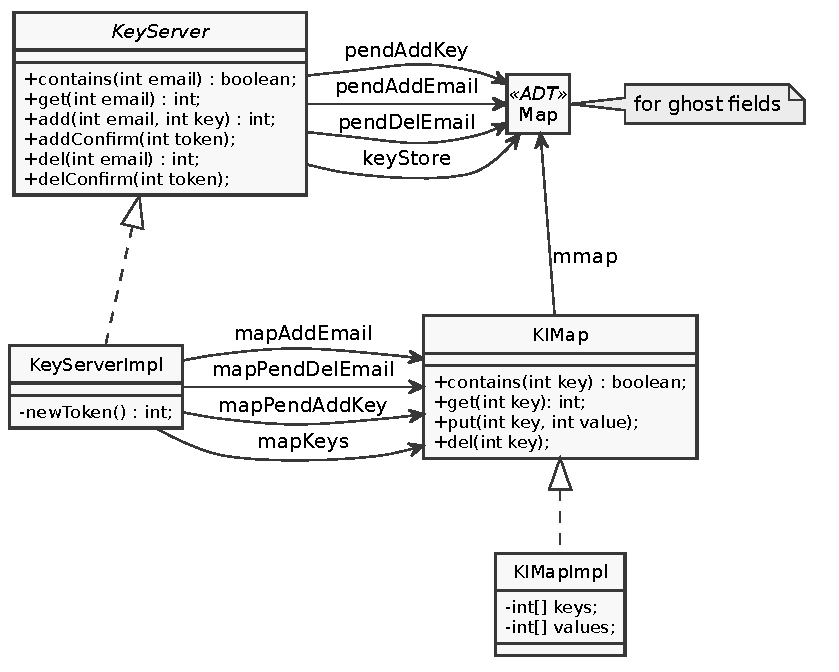
\includegraphics[height=.9\textheight]{imap}
\end{frame}

\begin{frame}[fragile]
  \frametitle{The map model}
\begin{lstlisting}
     /*@ public normal_behaviour
       @  requires true;
       @  ensures keyStore == \old(keyStore);
       @  ensures pendAddEmail == \dl_mapUpdate(\old(pendAddEmail), \result, id);
       @  ensures pendAddKey == \dl_mapUpdate(\old(pendAddKey), \result, pkey);
       @  ensures pendDelEmail == \old(pendDelEmail);
       @  ensures !\dl_inDomain(\old(pendAddEmail), \result);
       @  assignable footprint;
       @*/
    public int add(int id, int pkey);
\end{lstlisting}
\end{frame}


\begin{frame}[fragile]
  \frametitle{The map model}
\begin{lstlisting}[mathescape=true]
/*@ public normal_behaviour
  @  requires true;
  @  ensures keyStore == \old(keyStore);
  @  ensures pendAddEmail == \old(pendAddEmail)[\result := id];
  @  ensures pendAddKey == \old(pendAddKey)[\result := pkey];
  @  ensures pendDelEmail == \old(pendDelEmail);
  @  ensures !\result \in \old(pendAddEmail);
  @  assignable footprint;
  @*/
public int add(int id, int pkey);
\end{lstlisting}
\end{frame}

\begin{frame}[fragile]{The map model: Connection between ghost fields and implementation fields}
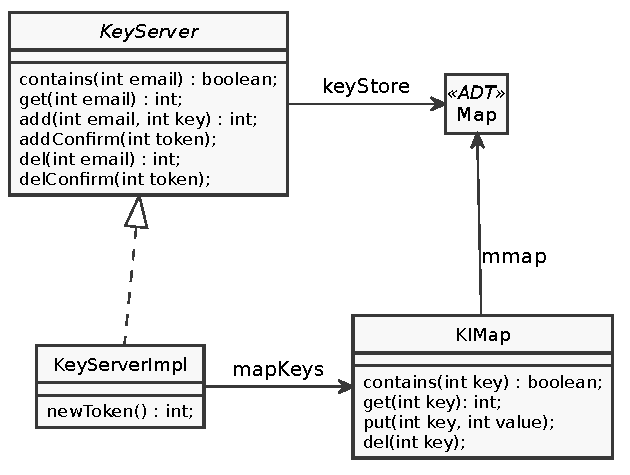
\includegraphics[width=7cm]{imap_partial}  
  
\begin{lstlisting}
interface KeyServer {
  //@ ghost \map keyStore;      /*...*/ 
}

class KeyServerImpl implements KeyServer {
    KIMap mapKeys = KIMap.newMap();
//@ invariant mapKeys.<inv>;
//@ invariant keyStore == mapKeys.mmap;
}
\end{lstlisting}
\end{frame}


\end{document}